\subsection{Results: Logistic Regression }
For logistic regression we see that learning rate, number of epochs and batch size affect accuracy differently. As we can see from Figure \ref{fig:LogRegLearningRate}, the model accuracy increases from the smallest learning rate up until the largest learning rate. The biggest accuracy achieved is about 91\% and the total increase is about 70\%. 

\begin{figure}[H]
    \centering
    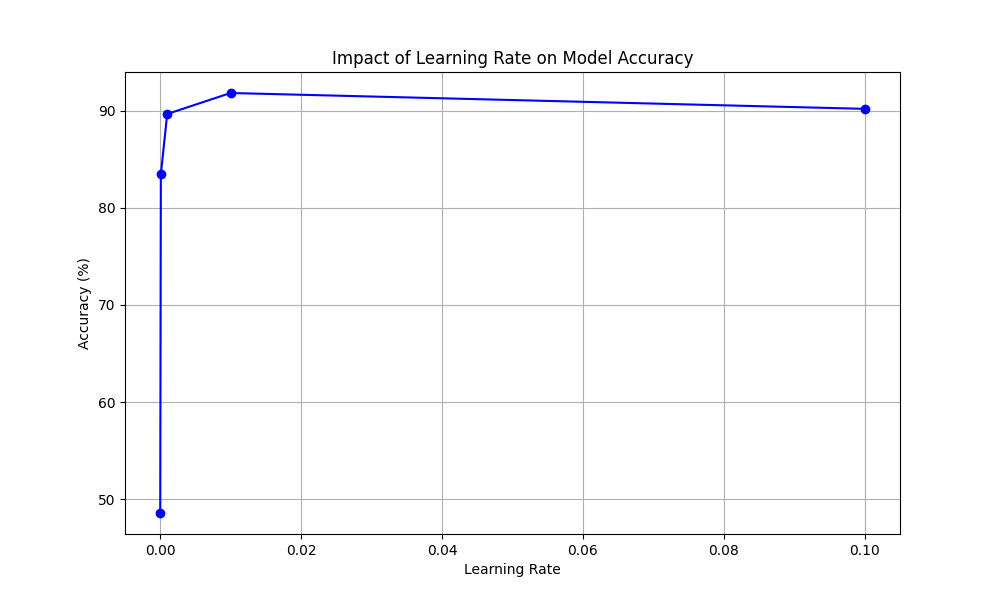
\includegraphics[width=\textwidth]{results/logreg/learning_rate_study.png}
    \caption{Logistic regression classification with learningrates in the range from $10^{-5}$ to $10^0$. The biggest accuracy is 91\% achieved with learning rate 0.1. }
    \label{fig:LogRegLearningRate}
\end{figure}

\newpage
From Figure \ref{fig:LogRegEpochs} we can see that number of epochs over 10 does not have any effect on accuracy. An accuracy of 91.4\% was achieved with all number of epochs except for 5 epochs were the accuracy is 90.6\%. It was considered to run more epochs but because of the diminishing returns when epochs increases we decided to save computational resources. 

\begin{figure}[H]
    \centering
    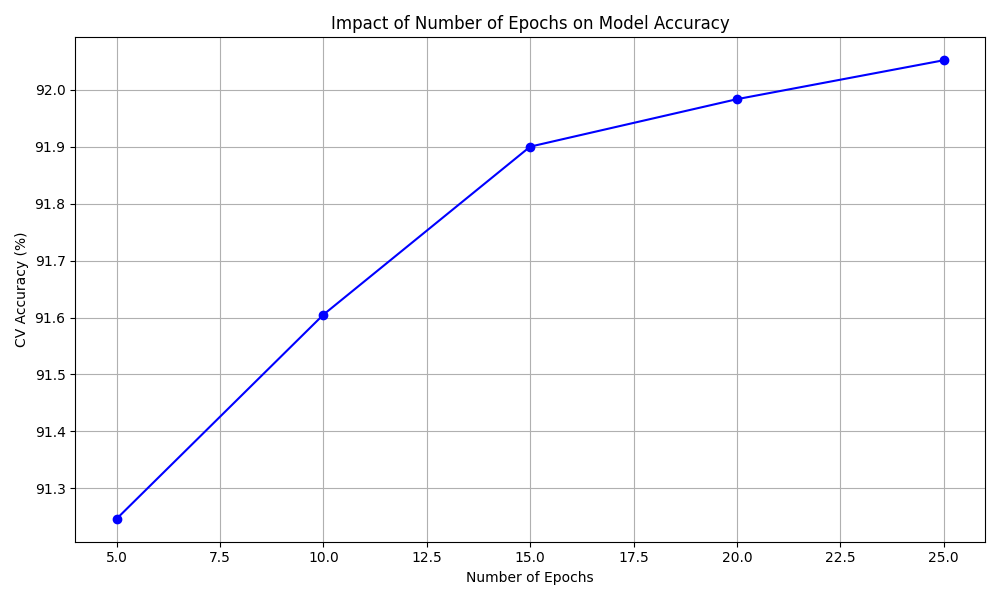
\includegraphics[width=\textwidth]{results/logreg/number_of_epochs_study.png}
    \caption{Logistic regression classification with epochs in the range from $5$ to $25$. The biggest accuracy achieved is 91.4\% with epochs above 10.}
    \label{fig:LogRegEpochs}
\end{figure}

\newpage
Moving on to Figure \ref{fig:LogRegBatchsize} we can see that in contrast to number of epochs, the increasing of batch size lowers accuracy. The biggest accuracy is 91.4\% when a batch size below 64 is used. It should be noted that the absolute value decrease of around 1\% for batch size and 0.8\% for epochs is not that big. This indicates that these two variables are less important in optimizing for accuracy than learning rate which had a 70\% difference from lowest to biggest. 

\begin{figure}[H]
    \centering
    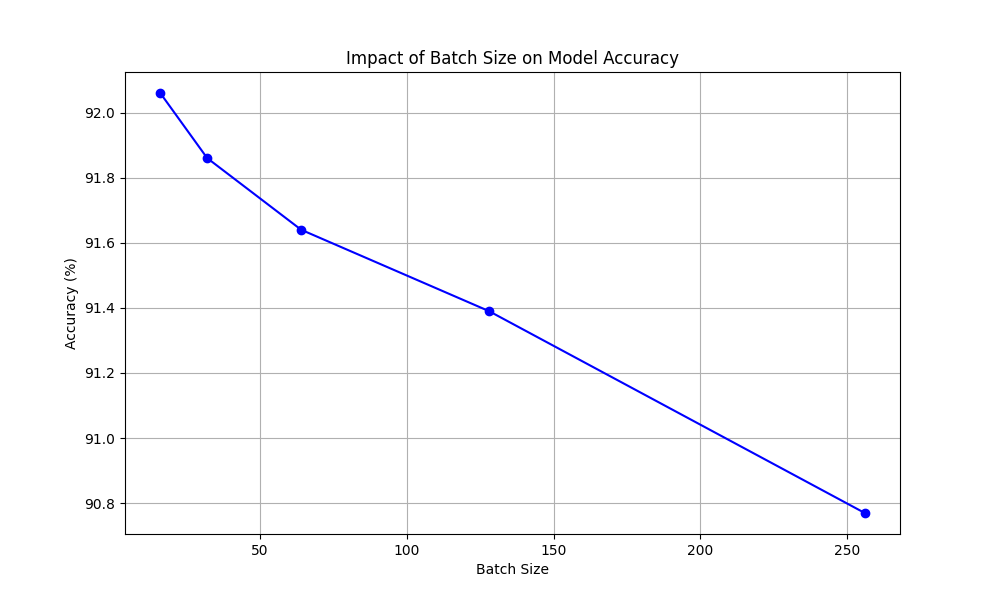
\includegraphics[width=\textwidth]{results/logreg/batch_size_study.png}
    \caption{Logistic regression classification with batchsize in the range from $16$ to $256$. The biggest accuracy achieved is 91.4\% when batch size is below 64.}
    \label{fig:LogRegBatchsize}
\end{figure}

\newpage
\subsection{Results: Grid search on CNN}
\subsubsection{Number of Linear Layers and Convolutional Layers}
From Figure \ref{fig:cnn:layers}, we found that an additional convolutional layer and an additional linear layer increase the accuracy by 0.2\% for our initial values. We decided to go on with this structure.
\begin{figure}[H]
    \centering
    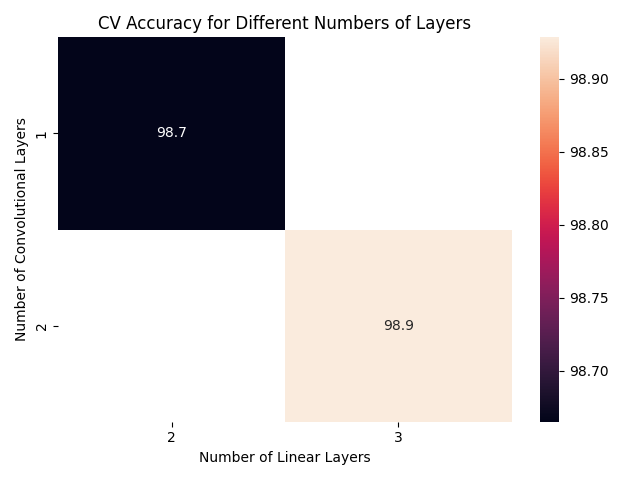
\includegraphics[width=\textwidth]{results/cnn_grid_search/heatmap_grid_search_layers.png}
    \caption{Results of a grid search comparing a convolutional neural network (CNN) with one convolutional layer followed by two linear layers, against a CNN with two convolutional layers followed by three linear layers.}
    \label{fig:cnn:layers}
\end{figure}

\newpage
\subsubsection{Kernel Size and Number of Filters}
Our results testing different kernel sizes and number of filters in each convolutional layers, illustrated in Figure \ref{fig:cnn_kf}, showed that our initial structure of (32, 64) filters gave the best performance. As the performance was equal for kernel size 5 and 7, we decided to continue with kernel size 5 as it is the simplest structure.
\begin{figure}[H]
    \centering
    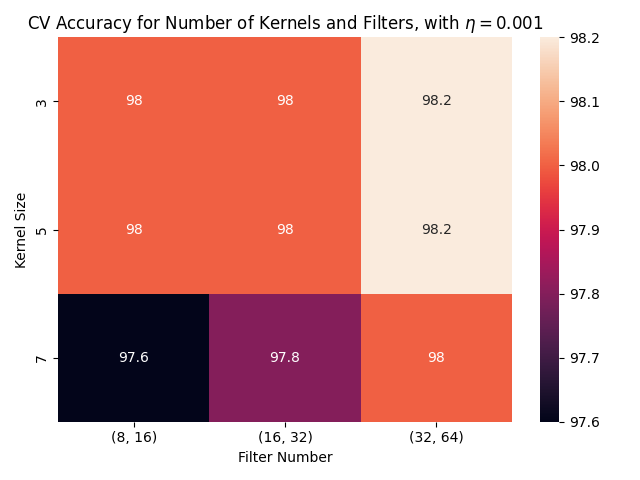
\includegraphics[width=\textwidth]{results/cnn_grid_search/heatmap_grid_search_kf.png}
    \caption{Results of a a grid search comparing differnent kernel sizes and number of filter in each of the two convolutional layers. Leraning rate is 0.001.}
    \label{fig:cnn_kf}
\end{figure}

\newpage
\subsubsection{Pooling and Padding}
\iris{THESE RESULTS NEED TESTING}
Pooling is good. Increased runtime significantly to not have it.
We continued with pooling. 

\begin{figure}[H]
    \centering
    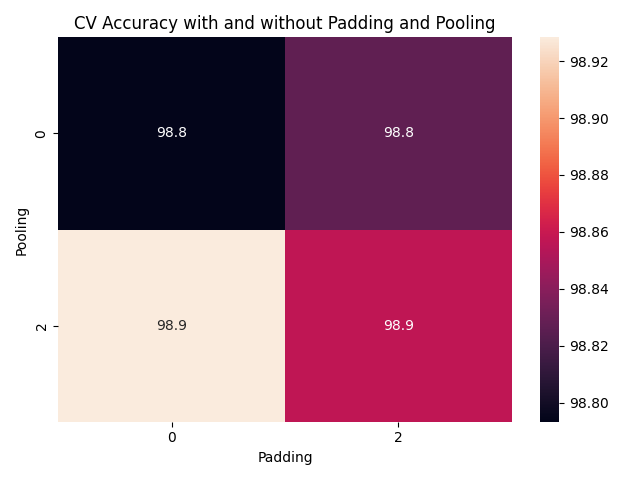
\includegraphics[width=\textwidth]{results/cnn_grid_search/heatmap_grid_search_pp.png}
    \caption{Results of a a grid search experimenting with adding padding and pooling after the convolutional layers \iris{is this correct?}}
    \label{fig:cnn_pp}
\end{figure}

\newpage
\subsubsection{Dropout Rates and Activation Functions}
 As we can see from Figure \ref{fig:cnn_pp} the accuracy does not change much depending on dropout rate and activation functions. When running the code for 10 epochs, we got 98\% accuracy for all four combinations. We suspected our model structure and training time was too simple/short to get an effect of the dropout rate, due to our model not being prone to overfit. When increasing the number of epochs to 20, we got the same accuracy of 98.2\% for LeakyRelu and Dropout rate 0.5. This is the same performance as our previous implementation with 10 epochs and no dropout. In line with our selection criterion, we decided to go keep our implementation with 10 epochs and no dropout layer, with Relu as the activation function. 

\begin{figure}[H]
    \centering
    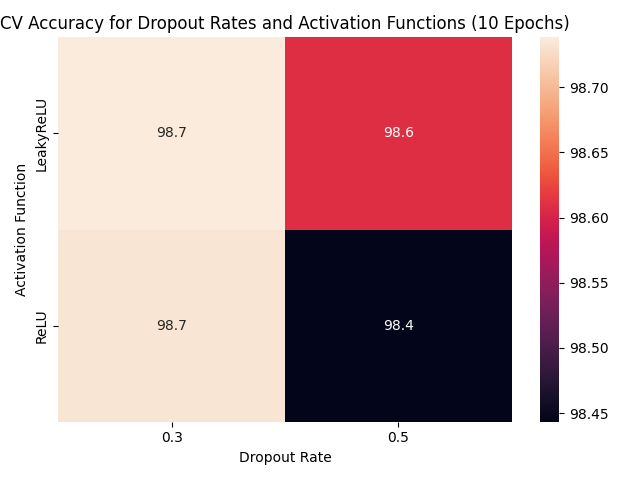
\includegraphics[width=\textwidth]{results/cnn_grid_search/heatmap_grid_search_da.png}
    \caption{Results of a a grid search experimenting with dropout rates and two different activation functions. We ran this result both with 10 and 20 epochs as we saw no change for 10 epochs, this plot is for 20 epochs. The results for 10 epochs can be found in the results folder of our code.}
    \label{fig:cnn_pp}
\end{figure}


\newpage
\subsection{Discussion of Performance}
The baseline vs CNN both reaches 90 \% without an extensive tuning of the baseline, which calls for the question if using convolutional neural networks are worth the trouble of runtime and reduced interpretability. However, in some applications of a model trained on the MNIST data set, such
as reading bank account numbers from handwritten digits, even tiny mistakes can be very costly.
Therefore, it is crucial to reduce this error as much as possible. \cite{raschka2022machine}

\iris {It should be noted that from the objective of performance, our tuning of hyperparameters could benefit from testing activation functions.}

A discussion: our results are highly sensitive to the initial values of our tuning. In a neural network, everything is interconnected, making it difficult to isolate individual effects. Earlier in this course, we spent considerable time examining how factors such as different learning rates, optimizers, and epochs influence learning convergence and model performance. In this project, however, we aimed to explore new hyper parameters specific to convolutional neural networks (CNNs): filter numbers, kernel size, dropout, padding, and pooling. Our focus on these new hyperparameters meant that we paid less attention to tuning the basic ones, which may have impacted our ability to achieve optimal model performance. For future work, we would like to explore more efficient methods of tuning neural networks, such as Bayesian optimization.

It was not fun to make a choice on the initial values, but we were forced to do it due to runtime. In the end we landed on making a choice we could argue, but in the perfect world we would test everything against each other. For computational resources, one could say that we chose a proper validation of the hyper parameters with cross-validation to take into account the randomness in different splits and model training, over testing everything against each other. 

\textbf{Critical assesment of the methods}
\iris{Draft below}
CNNs are not interpretable. Logreg is interpretable. It requires knowledge of various hyper parameters, and tuning og the hyper parameters. For the MNIST case, where you want to recognize digits, CNNs are worth the trouble for most obvious applications. But for other data sets with pictures

